
% ──────────────────────────────────────────────────────────────
\subsection{Inteligencia Artificial}
% ──────────────────────────────────────────────────────────────
 
La Inteligencia Artificial (IA) es la inteligencia llevada a cabo por máquinas, en la que un agente «inteligente» ideal percibe su entorno y lleva a cabo acciones que maximizan sus posibilidades de éxito en algún objetivo \parencite{bk_russell2009intart}. Este término se aplica cuando una máquina imita las funciones cognitivas que los seres humanos asocian con otras mentes, tales como aprender y resolver problemas \parencite{bk_russell2004intart}.
 
A lo largo de la historia se han seguido cuatro grandes enfoques: dos centrados en el comportamiento humano y dos enfocados en la racionalidad. El enfoque empírico nace con la prueba propuesta por Alan Turing en 1950, cuyo computador debía contar con capacidades de procesamiento de lenguaje natural, representación del conocimiento, razonamiento automático y aprendizaje automático. Si el evaluador incluía además una señal de video, la prueba pasaba a denominarse Prueba Global de Turing, sumando también visión computacional y robótica. Por su parte, el enfoque racional se fundamenta en las «leyes del pensamiento» enunciadas por filósofos griegos como Aristóteles, derivando en el estudio de la lógica y, posteriormente, en la tradición logista de la IA.
 
Actualmente, la IA cuenta con múltiples aplicaciones como la Minería de Datos, el Procesamiento de Lenguaje Natural (PLN), la robótica y los videojuegos. Dentro de ella se pueden encontrar ramas como el Aprendizaje Automático, la Visión Computacional y los Modelos de Lenguaje de Gran Escala, estas últimas de especial relevancia para la presente investigación.
 
% ──────────────────────────────────────────────────────────────
\subsection{Aprendizaje Automático}
% ──────────────────────────────────────────────────────────────
 
El Aprendizaje Automático (\textit{Machine Learning} en inglés) es una rama de la Inteligencia Artificial cuyo fin es desarrollar técnicas que permitan a las computadoras aprender mediante el hallazgo de algoritmos y heurísticas que conviertan muestras de datos en programas sin necesidad de programarlos explícitamente \parencite{bk_russell2009intart}. Sus algoritmos están compuestos por muchas tecnologías —como Aprendizaje Profundo, Redes Neuronales y Procesamiento de Lenguaje Natural— que operan guiadas por lecciones extraídas de información existente \parencite{bk_alpaydin2014ml}.
 
Los tres tipos de aprendizaje principales son el supervisado, el no supervisado y el por refuerzo. En el \textbf{aprendizaje supervisado}, se trabaja con datos etiquetados buscando obtener una función que asigne una respuesta de salida adecuada a partir de unos datos de entrada. Existen dos sub-tipos: la regresión, que obtiene como resultado un valor numérico continuo, y la clasificación, que asigna elementos a categorías discretas. En el \textbf{aprendizaje no supervisado}, se trabaja con datos no etiquetados para explorar la estructura latente de los datos mediante agrupamientos o \textit{clusters}. Finalmente, el \textbf{aprendizaje por refuerzo} consiste en que un agente aprende a tomar decisiones a partir de una retroalimentación denominada recompensa o refuerzo, lo que le permite optimizar una política de actuación a lo largo del tiempo.
 
% ──────────────────────────────────────────────────────────────
\subsection{Aprendizaje Profundo}
% ──────────────────────────────────────────────────────────────
 
El Aprendizaje Profundo (\textit{Deep Learning} en inglés) es un tipo de Aprendizaje Automático que entrena a una computadora para realizar tareas asociadas a los seres humanos —desde la identificación de imágenes hasta el reconocimiento del lenguaje— configurando parámetros básicos y entrenando al sistema para que aprenda por sí mismo reconociendo patrones mediante múltiples capas de procesamiento \parencite{gl_sas_deeplearning}. Se basa en teorías acerca de cómo funciona el cerebro humano, modelando redes de neuronas artificiales a gran escala.
 
La principal diferencia con el Aprendizaje Automático convencional es que el Aprendizaje Profundo realiza la extracción de características y la clasificación de manera simultánea, mientras que en el enfoque clásico estos procesos ocurren por separado. Esta característica lo convierte en la base tecnológica para los Modelos de Lenguaje de Gran Escala, que son el eje central de la presente investigación.
 
% ──────────────────────────────────────────────────────────────
\subsection{Procesamiento del Lenguaje Natural}
% ──────────────────────────────────────────────────────────────
 
El Procesamiento del Lenguaje Natural (\textit{Natural Language Processing}, NLP por sus siglas en inglés) es un campo interdisciplinario que combina lingüística computacional, ciencias de la computación, ciencia cognitiva e inteligencia artificial. Investiga el uso de computadoras para comprender el lenguaje humano con el fin de realizar tareas útiles, tales como reconocimiento de voz, análisis léxico, resumen automático de textos, análisis de sentimientos y detección de temas \parencite{bk_deng2018deeplearningnlp}.
 
Desde una perspectiva histórica, el NLP ha evolucionado a través de tres olas. El \textbf{Racionalismo} (décadas de 1960 a 1980) se fundamentó en reglas gramaticales diseñadas por expertos, basándose en la concepción del lenguaje como una facultad innata propuesta por Noam Chomsky. El \textbf{Empirismo} se caracterizó por la explotación de grandes corpus de texto mediante Aprendizaje Automático, con modelos como el Modelo Oculto de Markov (HMM). El \textbf{Aprendizaje Profundo}, como tercera y actual ola, emplea redes neuronales de múltiples capas entrenadas sobre volúmenes masivos de texto, permitiendo capturar dependencias semánticas complejas que los enfoques anteriores no podían modelar \parencite{bk_deng2018deeplearningnlp}.
 
Para el presente trabajo, el NLP constituye la disciplina madre que sustenta todas las técnicas aplicadas: el análisis de sentimientos, la detección de temas y los modelos de lenguaje de gran escala.
 
\subsubsection{Representación Vectorial del Texto}
 
Antes de aplicar cualquier modelo de NLP, el texto debe ser transformado en representaciones numéricas. Entre las modalidades más usadas se encuentran las siguientes.
 
La \textbf{Bolsa de Palabras} (\textit{Bag-of-Words} o BoW) extrae características de textos a partir de un vocabulario de palabras conocidas, cuantificando su frecuencia de aparición sin considerar el orden o la estructura de las palabras dentro del documento \parencite{bk_brownlee2017deeplearning_nlp}. La \textbf{Frecuencia del Término - Frecuencia Inversa del Documento} (\textit{TF-IDF}) resalta las palabras más significativas en el corpus al combinar la frecuencia de aparición de un término en un documento con la penalización de términos que aparecen en demasiados documentos, calculada mediante la Ecuación \ref{eq:tfidf_llm}:
 
\begin{equation}\label{eq:tfidf_llm}
\phantomsection
TF\text{-}IDF_{(t,d)} = TF_{(t,d)} \times \log\frac{N}{df_{(t)}}
\end{equation}
\myequations{Fórmula de TF-IDF para ponderación de términos}
 
Donde $TF_{(t,d)}$ es la frecuencia del término $t$ en el documento $d$, $N$ es el número total de documentos y $df_{(t)}$ es el número de documentos que contienen el término $t$.
 
La \textbf{Incrustación de Palabras} (\textit{Word Embedding}) representa las palabras como vectores densos de baja dimensionalidad en un espacio vectorial continuo, donde palabras con significados similares tienen representaciones cercanas. Algoritmos como Word2Vec \parencite{tec_mikolov2013word2vec} y GloVe \parencite{gl_pennington2014glove} popularizaron este enfoque. Sin embargo, estas representaciones son estáticas, es decir, una misma palabra tiene siempre el mismo vector independientemente del contexto en que aparezca. Los modelos de transformers, descritos más adelante, resuelven esta limitación al generar representaciones contextuales dinámicas.
 
% ──────────────────────────────────────────────────────────────
\subsection{La Arquitectura Transformer}
% ──────────────────────────────────────────────────────────────
 
La arquitectura Transformer, introducida por \cite{tec_vaswani2017attention} en el influyente artículo titulado «\textit{Attention Is All You Need}», representa el fundamento arquitectónico de todos los modelos de lenguaje modernos de gran escala. A diferencia de las Redes Neuronales Recurrentes (RNN) y las Redes de Memoria Larga a Corto Plazo (LSTM), el Transformer prescinde de la recurrencia y procesa la secuencia de entrada completa en paralelo mediante un mecanismo denominado \textit{self-attention} (auto-atención), lo que permite capturar dependencias de largo alcance entre palabras de manera mucho más eficiente.
 
\subsubsection{Mecanismo de Atención}
 
El mecanismo central del Transformer es la \textbf{atención multi-cabeza} (\textit{multi-head attention}). Este mecanismo calcula, para cada token (unidad léxica) de la secuencia, cuánta «atención» debe prestarse a cada otro token al momento de construir su representación. Formalmente, la atención se define mediante la Ecuación \ref{eq:attention}:
 
\begin{equation}\label{eq:attention}
\phantomsection
\text{Attention}(Q, K, V) = \text{softmax}\left(\frac{QK^T}{\sqrt{d_k}}\right)V
\end{equation}
\myequations{Fórmula del mecanismo de atención escalada por producto punto}
 
Donde:
\begin{conditions}
Q   & matriz de consultas (\textit{queries}) \\
K   & matriz de claves (\textit{keys}) \\
V   & matriz de valores (\textit{values}) \\
d_k & dimensión de los vectores de claves
\end{conditions}
 
El producto $QK^T$ mide la similitud entre cada par de tokens; dividir entre $\sqrt{d_k}$ estabiliza los gradientes durante el entrenamiento; y la función \textit{softmax} convierte los puntajes en una distribución de probabilidad sobre todos los tokens. Finalmente, los valores $V$ son ponderados por estos pesos de atención. Este proceso se ejecuta en paralelo para múltiples «cabezas» de atención, cada una aprendiendo distintos tipos de relaciones semánticas y sintácticas entre los tokens.
 
\subsubsection{Arquitectura Encoder-Decoder}
 
El Transformer original sigue una arquitectura codificador-decodificador (\textit{encoder-decoder}), ilustrada en la Figura \ref{fig:transformer_arch}. El \textbf{codificador} (\textit{encoder}) procesa la secuencia de entrada y genera representaciones contextuales de alta dimensión. El \textbf{decodificador} (\textit{decoder}) toma estas representaciones junto con la secuencia generada hasta el momento para producir el siguiente token de salida, de manera autoregresiva.
 
\begin{figure}[!ht]
    \begin{center}
        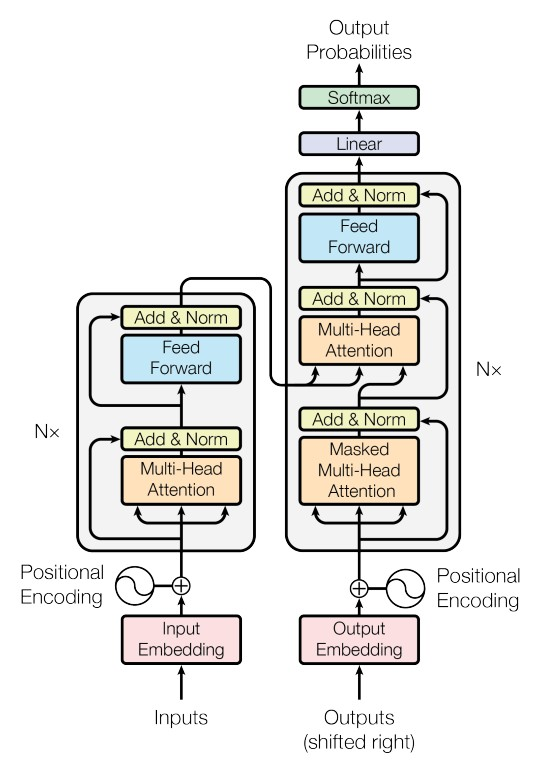
\includegraphics[width=0.70\textwidth]{2/figures/transformer_architecture.jpg}
        \caption[Arquitectura original del Transformer con codificador y decodificador]{Arquitectura original del modelo Transformer, compuesta por un codificador (izquierda) y un decodificador (derecha), cada uno formado por capas de atención multi-cabeza y redes de retroalimentación.\\
            Fuente: \cite{tec_vaswani2017attention}. \textit{Attention Is All You Need}. (p. 3)}
        \label{fig:transformer_arch}
    \end{center}
\end{figure}
 
Existen variantes especializadas: los modelos \textbf{solo-encoder} (como BERT) son óptimos para tareas de comprensión y clasificación de texto, los modelos \textbf{solo-decoder} (como GPT) son óptimos para generación de texto, y los modelos \textbf{encoder-decoder} (como T5) son ideales para tareas de transformación de secuencias como la traducción automática o el resumen. Esta distinción es fundamental para comprender la familia de LLMs utilizados en la presente investigación.
 
% ──────────────────────────────────────────────────────────────
\subsection{Modelos de Lenguaje de Gran Escala (LLMs)}
% ──────────────────────────────────────────────────────────────
 
Los Modelos de Lenguaje de Gran Escala (\textit{Large Language Models}, LLMs) son modelos basados en la arquitectura Transformer, pre-entrenados sobre corpus de texto de escala masiva —que pueden abarcar billones de tokens— con el objetivo de aprender representaciones ricas y generalizables del lenguaje \parencite{bk_russell2009intart}. Su denominación como «de gran escala» hace referencia tanto al volumen de datos de entrenamiento como al número de parámetros del modelo, que en los casos más avanzados supera los 100 mil millones.
 
\subsubsection{Pre-entrenamiento y Ajuste Fino}
 
El ciclo de vida de un LLM comprende dos etapas principales. En la etapa de \textbf{pre-entrenamiento}, el modelo aprende a predecir tokens a partir de grandes corpus no etiquetados mediante objetivos de aprendizaje auto-supervisado, como la predicción de la siguiente palabra (\textit{next-token prediction}) en modelos GPT o el enmascaramiento de tokens (\textit{masked language modeling}) en modelos BERT \parencite{tec_devlin2018bert}. Esta etapa dota al modelo de conocimiento lingüístico y factual amplio pero general.
 
En la etapa de \textbf{ajuste fino} (\textit{fine-tuning}), el modelo pre-entrenado se re-entrena sobre un conjunto de datos etiquetado y específico de la tarea objetivo —como clasificación de sentimientos políticos o detección de temas electorales— adaptando sus parámetros al dominio concreto de aplicación. Existe además el ajuste fino con instrucciones (\textit{instruction fine-tuning}) y con retroalimentación humana (\textit{Reinforcement Learning from Human Feedback}, RLHF), técnicas que han sido clave en la alineación de modelos como GPT-4 y Claude \parencite{tec_ouyang2022instructgpt}.
 
\subsubsection{Aprendizaje por Contexto: Zero-shot y Few-shot}
 
Una capacidad emergente de los LLMs de gran escala es el \textbf{aprendizaje por contexto} (\textit{in-context learning}), que permite al modelo realizar nuevas tareas sin actualizar sus parámetros, simplemente incluyendo ejemplos o instrucciones en el \textit{prompt} (texto de entrada). Se distinguen dos modalidades principales, representadas en la Figura \ref{fig:zeroshot_fewshot}:
 
\begin{figure}[!ht]
    \begin{center}
        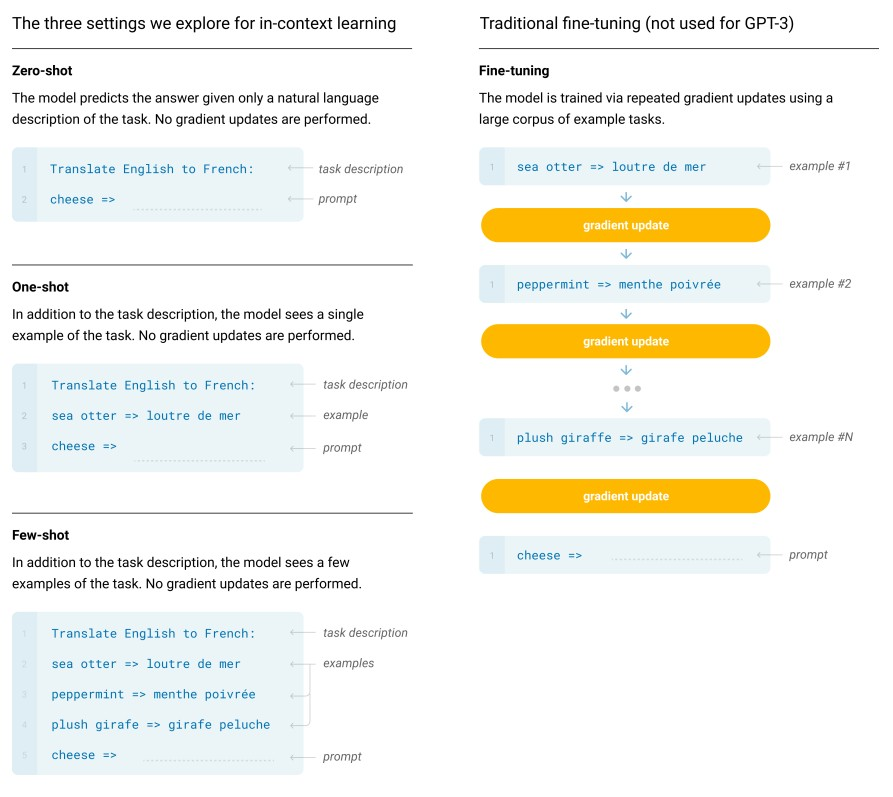
\includegraphics[width=0.88\textwidth]{2/figures/zeroshot_fewshot.jpg}
        \caption[Comparación entre los enfoques zero-shot, one-shot y few-shot en LLMs]{Comparación entre los paradigmas zero-shot, one-shot y few-shot para el aprendizaje por contexto en modelos de lenguaje de gran escala.\\
            Fuente: \cite{tec_brown2020gpt3}. \textit{Language Models are Few-Shot Learners}. (p. 7)}
        \label{fig:zeroshot_fewshot}
    \end{center}
\end{figure}
 
\begin{itemize}
    \item \textbf{Zero-shot}: El modelo realiza la tarea sin recibir ningún ejemplo previo, únicamente con una descripción de la tarea en el \textit{prompt}. Esta modalidad es especialmente útil cuando no se dispone de datos etiquetados en el dominio objetivo.
    \item \textbf{Few-shot}: El modelo recibe un pequeño número de ejemplos etiquetados en el \textit{prompt} antes de procesar la consulta real. Esta modalidad mejora significativamente el desempeño en tareas especializadas sin necesidad de re-entrenamiento.
\end{itemize}
 
Ambas modalidades son fundamentales en la presente investigación, ya que permiten aplicar LLMs al análisis de discurso político sin requerir grandes conjuntos de datos etiquetados en español.
 
\subsubsection{Modelos LLM Relevantes para la Investigación}
 
Varios LLMs son directamente relevantes para los objetivos de esta tesis:
 
\textbf{BERT} (\textit{Bidirectional Encoder Representations from Transformers}), propuesto por \cite{tec_devlin2018bert}, es un modelo solo-encoder que introduce el pre-entrenamiento bidireccional, permitiendo capturar el contexto tanto izquierdo como derecho de cada token simultáneamente. Ha sido ampliamente adoptado para clasificación de sentimientos y tareas de comprensión textual.
 
\textbf{RoBERTa} (\textit{Robustly Optimized BERT Pretraining Approach}) es una versión optimizada de BERT que emplea mayor volumen de datos y elimina el objetivo de predicción de oración siguiente (\textit{next sentence prediction}), logrando mejoras significativas en benchmarks de NLP \parencite{tec_liu2019roberta}.
 
\textbf{GPT} (\textit{Generative Pre-trained Transformer}) es una familia de modelos solo-decoder desarrollados por OpenAI, siendo GPT-3 \parencite{tec_brown2020gpt3} el primero en demostrar capacidades emergentes de aprendizaje few-shot a gran escala, y GPT-4 su sucesor de mayor capacidad.
 
\textbf{Llama} es una familia de LLMs de código abierto desarrollada por Meta AI \parencite{tec_touvron2023llama}, que ha democratizado la investigación con LLMs al ofrecer modelos de alto rendimiento sin restricciones de acceso. Su variante Llama~2 ha sido ampliamente utilizada en estudios de análisis político descritos en los antecedentes de esta investigación.
 
La Figura \ref{fig:llm_timeline} ilustra la evolución cronológica de los principales LLMs desde 2018 hasta la actualidad, evidenciando la aceleración en el desarrollo de estos modelos y el exponencial crecimiento en su número de parámetros.
 
\begin{figure}[!ht]
    \begin{center}
        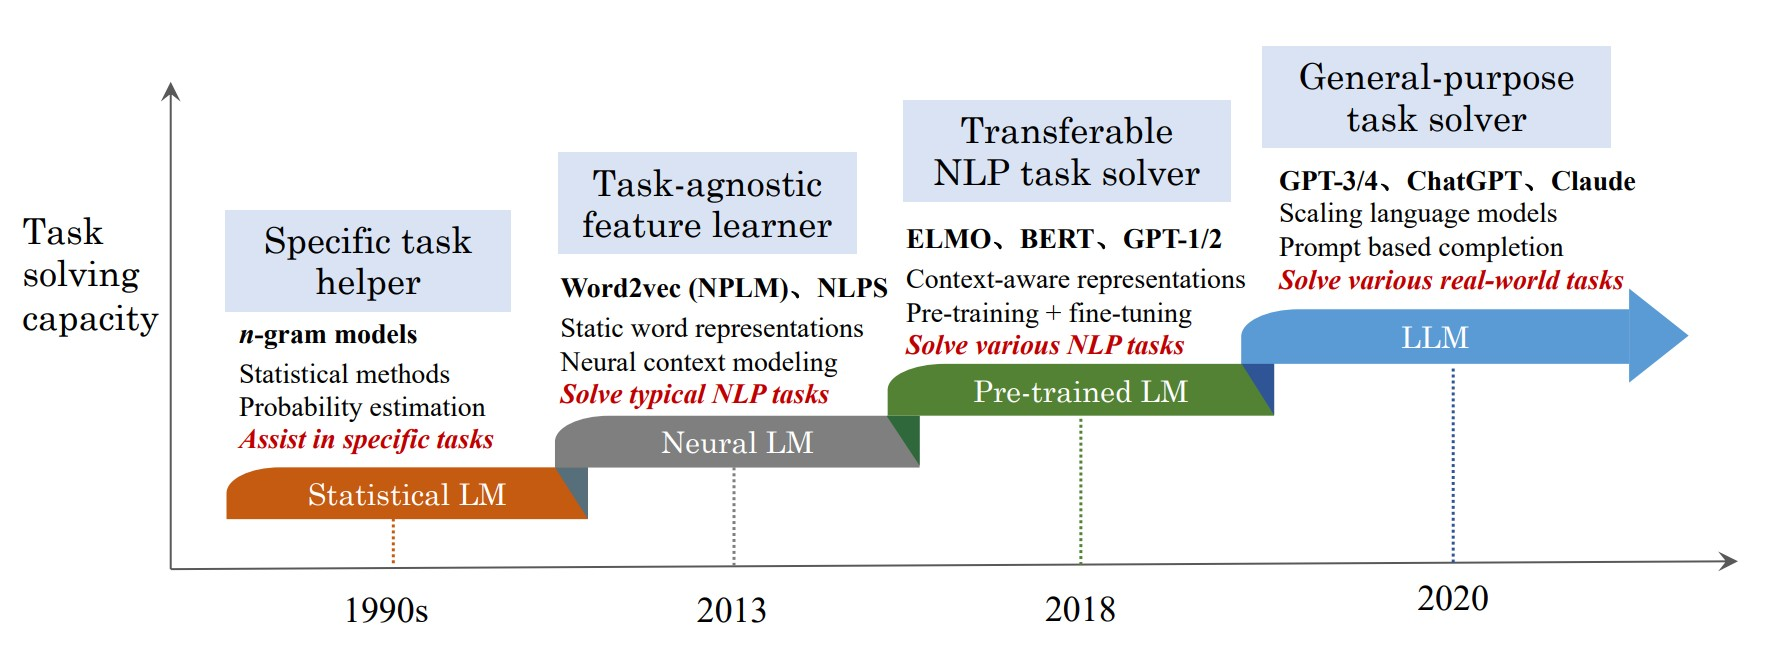
\includegraphics[width=0.92\textwidth]{2/figures/llm_timeline.jpg}
        \caption[Evolución cronológica de los principales modelos de lenguaje de gran escala]{Línea de tiempo de los principales LLMs, mostrando el crecimiento exponencial en número de parámetros y capacidades.\\
        Fuente: \cite{tec_zhao2023llm_survey}. \citetitle{tec_zhao2023llm_survey}. (p. 2)}
        \label{fig:llm_timeline}
    \end{center}
\end{figure}
 
% ──────────────────────────────────────────────────────────────
\subsection{Análisis de Sentimientos}
% ──────────────────────────────────────────────────────────────
 
El análisis de sentimientos, también denominado minería de opiniones (\textit{opinion mining}), es la tarea de NLP orientada a identificar y extraer información subjetiva de textos, determinando si el contenido expresa una actitud positiva, negativa o neutral hacia una entidad, persona, evento o tema \parencite{tec_liu2012sentiment}. En el contexto de la inteligencia electoral, esta tarea permite medir la percepción pública hacia candidatos, partidos políticos y políticas públicas a partir de grandes volúmenes de publicaciones en ecosistemas digitales.
 
\subsubsection{Niveles de Análisis}
 
El análisis de sentimientos puede realizarse en distintos niveles de granularidad, como se ilustra en la Figura \ref{fig:sentiment_levels}:
 
\begin{figure}[!ht]
    \begin{center}
        \includegraphics[width=0.85\textwidth]{2/figures/sentiment_levels.jpg}
        \caption[Niveles de granularidad del análisis de sentimientos]{Niveles de análisis de sentimientos: a nivel de documento, a nivel de oración y a nivel de aspecto, con sus respectivos ejemplos de aplicación en textos políticos.\\
            Fuente: Elaboración propia basada en \cite{tec_liu2012sentiment}.}
        \label{fig:sentiment_levels}
    \end{center}
\end{figure}
 
\begin{itemize}
    \item \textbf{Nivel de documento}: Se asigna una polaridad global al documento completo. Es el nivel más simple pero pierde información sobre aspectos específicos mencionados en el texto.
    \item \textbf{Nivel de oración}: Se analiza el sentimiento de cada oración de forma independiente, permitiendo una granularidad mayor.
    \item \textbf{Nivel de aspecto} (\textit{Aspect-Based Sentiment Analysis}, ABSA): Se identifica el sentimiento expresado hacia entidades o aspectos específicos mencionados en el texto. Por ejemplo, en un tweet sobre una campaña electoral, se puede detectar sentimiento positivo hacia la propuesta económica de un candidato y negativo hacia su gestión en seguridad.
\end{itemize}
 
\subsubsection{Enfoques Metodológicos}
 
Los principales enfoques para el análisis de sentimientos son los siguientes:
 
El \textbf{enfoque basado en léxicos} utiliza diccionarios de palabras con polaridad pre-asignada (por ejemplo, VADER, SentiWordNet, AFINN) para calcular el sentimiento de un texto mediante la suma de las puntuaciones de sus palabras. Es rápido y no requiere datos de entrenamiento, pero tiene dificultades con el lenguaje figurado, la ironía y el sarcasmo, tan frecuentes en el discurso político.
 
El \textbf{enfoque basado en aprendizaje automático supervisado} entrena clasificadores como Naive Bayes, SVM o Regresión Logística sobre conjuntos de datos etiquetados. Supera al anterior en precisión pero requiere datos etiquetados en el dominio y el idioma objetivo.
 
El \textbf{enfoque basado en Aprendizaje Profundo y LLMs} utiliza modelos como BERT, RoBERTa o GPT para generar representaciones contextuales del texto, logrando los mejores resultados en la actualidad. La Figura \ref{fig:sentiment_comparison} ilustra la comparación de rendimiento entre estos enfoques en tareas de análisis de sentimientos políticos.
 
\begin{figure}[!ht]
    \begin{center}
        \includegraphics[width=0.82\textwidth]{2/figures/sentiment_comparison.jpg}
        \caption[Comparación de rendimiento entre enfoques de análisis de sentimientos en texto político]{Comparación de exactitud entre los enfoques léxico, aprendizaje automático clásico y modelos basados en LLMs para análisis de sentimientos en texto político en redes sociales.\\
            Fuente: Elaboración propia basada en \cite{tec_liu2012sentiment} y \cite{pr_alvarez2023llm_political}.}
        \label{fig:sentiment_comparison}
    \end{center}
\end{figure}
 
\subsubsection{Desafíos en el Análisis de Sentimientos Político}
 
El análisis de sentimientos aplicado al discurso político en ecosistemas digitales presenta desafíos específicos que los métodos convencionales no resuelven satisfactoriamente. En primer lugar, el \textbf{lenguaje figurado}: la ironía, el sarcasmo y el humor político son formas frecuentes de expresión en redes sociales, y su interpretación requiere comprender el contexto pragmático más allá del significado literal de las palabras. En segundo lugar, la \textbf{ambigüedad de entidades}: un mismo tweet puede expresar sentimientos positivos hacia un partido y negativos hacia otro, o referirse a múltiples figuras políticas simultáneamente. En tercer lugar, la \textbf{diversidad lingüística}: en contextos latinoamericanos, el español presenta variaciones léxicas y expresivas significativas entre países, lo que dificulta la generalización de modelos entrenados en una sola variedad. Los LLMs multilingües como XLM-RoBERTa han mostrado ventajas sustanciales para este tipo de escenarios.
 
% ──────────────────────────────────────────────────────────────
\subsection{Detección Dinámica de Temas}
% ──────────────────────────────────────────────────────────────
 
La detección de temas (\textit{topic modeling} o \textit{topic detection}) es una familia de técnicas de NLP no supervisadas cuyo objetivo es descubrir automáticamente los temas o asuntos latentes que subyacen en un corpus de documentos, sin necesidad de etiquetas previas \parencite{bk_blei2012lda}. En el contexto de la inteligencia electoral, permite identificar qué temas están siendo discutidos en el ecosistema digital político, con qué intensidad y cómo evolucionan en el tiempo.
 
\subsubsection{Modelos Probabilísticos: LDA}
 
La \textbf{Asignación Latente de Dirichlet} (\textit{Latent Dirichlet Allocation}, LDA), propuesta por \cite{bk_blei2012lda}, es el modelo de detección de temas más influyente de la era pre-transformers. LDA asume que cada documento es una mezcla de temas, y que cada tema es una distribución de probabilidad sobre palabras. El proceso generativo de LDA se representa en la Figura \ref{fig:lda_plate}.
 
\begin{figure}[!ht]
    \begin{center}
        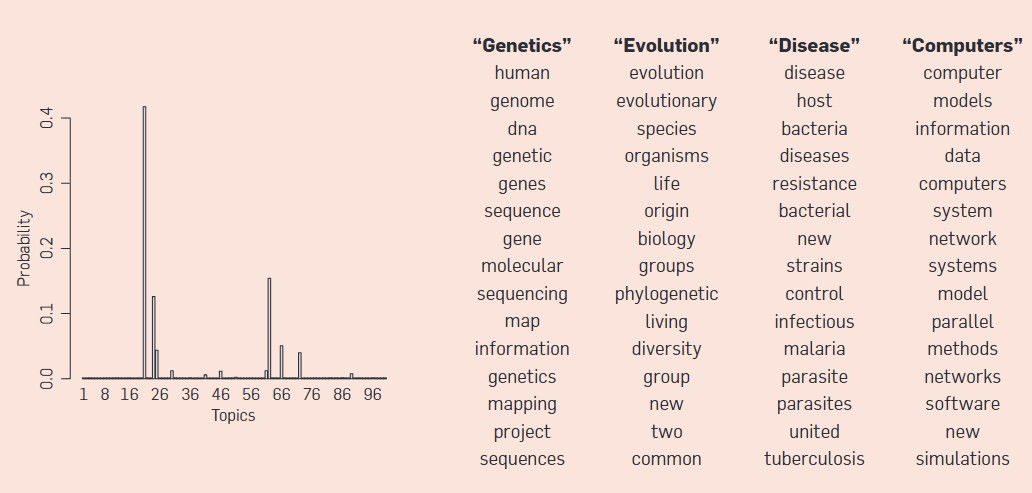
\includegraphics[width=0.70\textwidth]{2/figures/lda_plate.jpg}
        \caption[Notación de plato del modelo LDA]{Notación de plato del modelo de Asignación Latente de Dirichlet (LDA), mostrando las distribuciones de temas por documento ($\theta$) y de palabras por tema ($\phi$), controladas por los hiperparámetros Dirichlet $\alpha$ y $\beta$.\\
            Fuente: \cite{bk_blei2012lda}. \textit{Probabilistic Topic Models}. (p. 79)}
        \label{fig:lda_plate}
    \end{center}
\end{figure}
 
Sin embargo, LDA presenta limitaciones importantes para el análisis de datos de redes sociales: sus representaciones de topics son locales y no contextuales, tiene dificultades con textos muy cortos como tweets, y no puede capturar temas emergentes en tiempo real sin re-entrenamiento completo del modelo.
 
\subsubsection{BERTopic: Modelado de Temas Neural}
 
\textbf{BERTopic}, propuesto por \cite{tec_grootendorst2022bertopic}, es un framework moderno de modelado de temas que aprovecha embeddings de transformers y clustering basado en densidad. Su pipeline se compone de cuatro etapas principales, representadas en la Figura \ref{fig:bertopic_pipeline}:
 
\begin{figure}[!ht]
    \begin{center}
        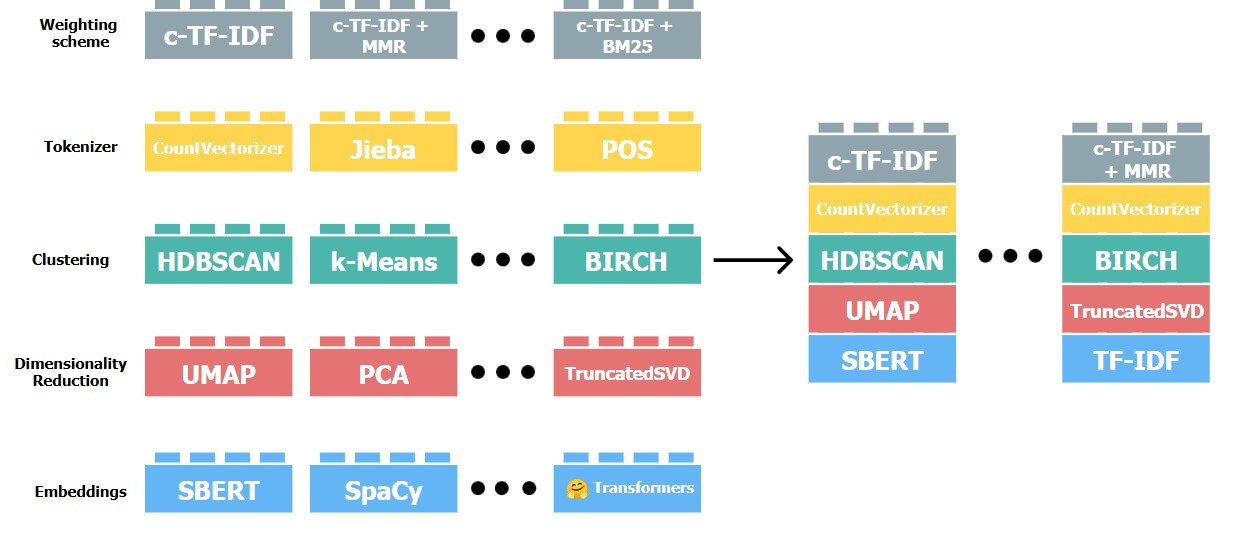
\includegraphics[width=0.90\textwidth]{2/figures/bertopic_pipeline.jpg}
        \caption[Pipeline completo del framework BERTopic para detección de temas neurales]{Pipeline del framework BERTopic: generación de embeddings con transformers, reducción de dimensionalidad con UMAP, clustering con HDBSCAN y representación de temas con c-TF-IDF.\\
            Fuente: \cite{tec_grootendorst2022bertopic}. \textit{BERTopic: Neural Topic Modeling with a Class-Based TF-IDF Procedure}.}
        \label{fig:bertopic_pipeline}
    \end{center}
\end{figure}
 
\begin{enumerate}
    \item \textbf{Generación de embeddings}: Cada documento es transformado en un vector de alta dimensión mediante un modelo de transformers (generalmente Sentence-BERT), capturando su significado semántico completo en contexto.
    \item \textbf{Reducción de dimensionalidad}: Los embeddings de alta dimensión son reducidos mediante UMAP (\textit{Uniform Manifold Approximation and Projection}), preservando la estructura local del espacio semántico.
    \item \textbf{Clustering}: El algoritmo HDBSCAN (\textit{Hierarchical Density-Based Spatial Clustering of Applications with Noise}) agrupa los documentos en clusters sin requerir especificar el número de grupos a priori, asignando automáticamente los documentos ruidosos o atípicos a la categoría de «outliers».
    \item \textbf{Representación de temas}: Cada cluster de documentos es representado mediante una variante de c-TF-IDF (\textit{class-based TF-IDF}), que identifica las palabras más características de ese grupo de documentos en relación al resto del corpus.
\end{enumerate}
 
BERTopic supera a LDA en coherencia semántica, manejo de textos cortos y capacidad de integración con LLMs para la generación de etiquetas interpretables para cada tema \parencite{tec_grootendorst2022bertopic}.
 
\subsubsection{Detección Dinámica de Temas}
 
La \textbf{detección dinámica de temas} (\textit{dynamic topic modeling}) extiende los modelos estáticos para rastrear cómo los temas evolucionan a través del tiempo. BERTopic implementa esta capacidad mediante la segmentación temporal del corpus: los documentos se agrupan en ventanas de tiempo y se re-calculan las representaciones de topics para cada período, permitiendo visualizar la evolución de narrativas políticas en el tiempo, como se muestra en la Figura \ref{fig:dynamic_topics}.
 
\begin{figure}[!ht]
    \begin{center}
        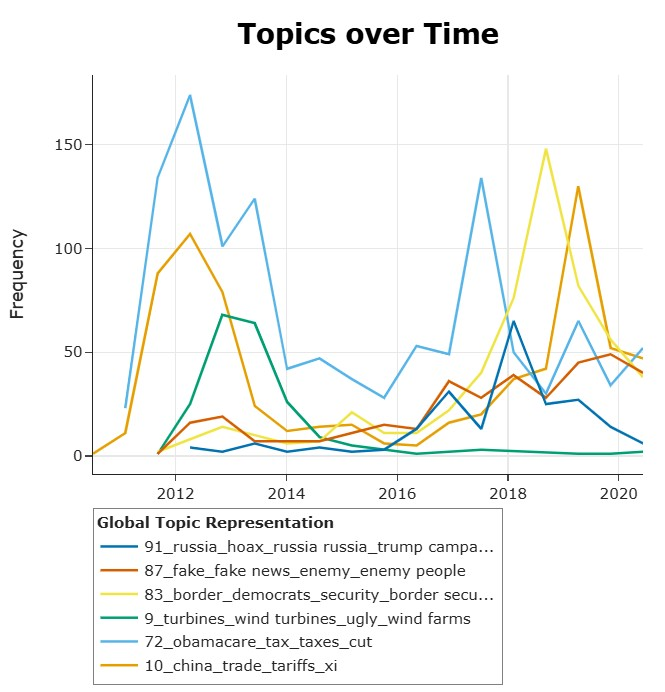
\includegraphics[width=0.88\textwidth]{2/figures/dynamic_topics.jpg}
        \caption[Evolución temporal de temas políticos detectados mediante BERTopic dinámico]{Ejemplo de evolución temporal de temas políticos detectados mediante el módulo de topic modeling dinámico de BERTopic, mostrando la frecuencia relativa de cada tema por período de tiempo.\\
            Fuente: \cite{tec_grootendorst2022bertopic}. \textit{BERTopic: Neural Topic Modeling with a Class-Based TF-IDF Procedure}.}
        \label{fig:dynamic_topics}
    \end{center}
\end{figure}
 
Esta capacidad es fundamental para los objetivos de la presente investigación, ya que el ecosistema digital durante un proceso electoral es altamente dinámico: los temas de campaña emergen, se intensifican y decaen en función de eventos como debates, escándalos o anuncios de política pública.
 
% ──────────────────────────────────────────────────────────────
\subsection{Ingeniería de Prompts}
% ──────────────────────────────────────────────────────────────
 
La \textbf{ingeniería de \textit{prompts}} (\textit{prompt engineering}) es la disciplina que estudia el diseño y optimización de las instrucciones textuales (\textit{prompts}) que se proporcionan a los LLMs para obtener de ellos respuestas de mayor calidad, precisión y relevancia sin modificar los parámetros del modelo \parencite{tec_white2023prompt}. En el contexto de la inteligencia electoral, el diseño adecuado de prompts determina en gran medida la calidad del análisis de sentimientos y la detección de temas que produce el LLM.
 
\subsubsection{Principales Técnicas}
 
Entre las técnicas de prompting más relevantes para esta investigación se encuentran las siguientes.
 
El \textbf{Chain-of-Thought prompting} (CoT) consiste en incluir en el \textit{prompt} una cadena de pasos de razonamiento intermedios antes de la respuesta final, lo cual mejora el desempeño de los LLMs en tareas que requieren razonamiento complejo \parencite{tec_wei2022cot}. Por ejemplo, en la clasificación de sentimientos políticos, se le puede pedir al modelo que primero identifique las entidades mencionadas, luego los términos evaluativos y finalmente el sentimiento hacia cada entidad.
 
El \textbf{Role prompting} asigna al LLM un rol específico al inicio del \textit{prompt} («Eres un analista político experto en discurso electoral latinoamericano...»), orientando sus respuestas hacia el dominio de interés. Esta técnica ha demostrado ser efectiva para mejorar la precisión en tareas de análisis político \parencite{pr_alvarez2023llm_political}.
 
La \textbf{Generación Aumentada por Recuperación} (\textit{Retrieval-Augmented Generation}, RAG) complementa el \textit{prompt} con información recuperada de una base de conocimiento externa (documentos de prensa, bases de datos electorales, programas de gobierno), permitiendo al LLM razonar sobre información actualizada y específica del dominio que puede no estar en sus datos de entrenamiento \parencite{tec_lewis2020rag}. La Figura \ref{fig:rag_architecture} ilustra la arquitectura general de un sistema RAG.
 
\begin{figure}[!ht]
    \begin{center}
        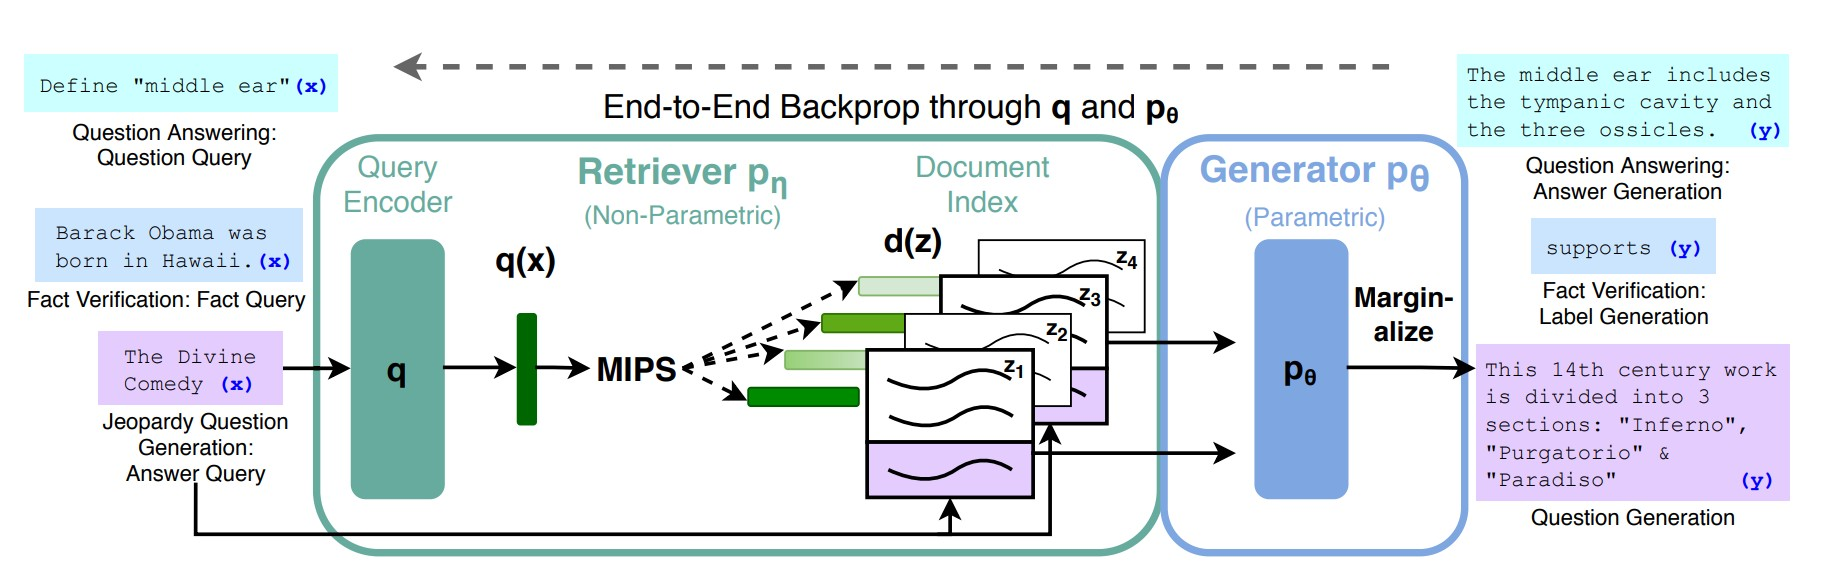
\includegraphics[width=0.88\textwidth]{2/figures/rag_architecture.jpg}
        \caption[Arquitectura de un sistema de Generación Aumentada por Recuperación (RAG)]{Arquitectura de un sistema RAG aplicado al análisis de discurso político: el módulo de recuperación obtiene documentos relevantes de una base de conocimiento externa, que son incluidos en el \textit{prompt} junto a la consulta del usuario para que el LLM genere una respuesta fundamentada.\\
            Fuente: \cite{tec_lewis2020rag}. \textit{Retrieval-Augmented Generation for Knowledge-Intensive NLP Tasks}. (p. 3)}
        \label{fig:rag_architecture}
    \end{center}
\end{figure}
 
% ──────────────────────────────────────────────────────────────
\subsection{Ecosistemas Digitales y Redes Sociales como Fuente de Datos}
% ──────────────────────────────────────────────────────────────
 
Los \textbf{ecosistemas digitales} son entornos mediáticos complejos conformados por la interacción de múltiples plataformas digitales —redes sociales, sitios de noticias, foros, aplicaciones de mensajería— a través de las cuales los ciudadanos producen, consumen y difunden información política \parencite{tec_chadwick2013hybrid}. En el contexto electoral, estos ecosistemas constituyen la principal arena de debate político contemporáneo, superando en muchos aspectos a los medios tradicionales en velocidad, alcance e interactividad.
 
Las \textbf{redes sociales} como X (antes Twitter), Facebook, TikTok e Instagram son las fuentes de datos primarias para los sistemas de inteligencia electoral. X/Twitter, en particular, ha sido ampliamente utilizada en la investigación académica por su naturaleza pública y la disponibilidad de su API, que permite la recolección masiva de datos geolocalizados y temporalmente etiquetados \parencite{pr_alvi2023twitter_election_review}. Sus características estructurales —textos cortos (hasta 280 caracteres), hashtags, menciones de usuarios y retweets— la convierten en una fuente especialmente rica para el análisis de sentimientos y la detección de temas en tiempo real.
 
\subsubsection{Recolección y Procesamiento de Datos de Redes Sociales}
 
La recolección de datos de redes sociales para análisis electoral generalmente sigue el proceso ilustrado en la Figura \ref{fig:data_collection_pipeline}:
 
\begin{figure}[!ht]
    \begin{center}
        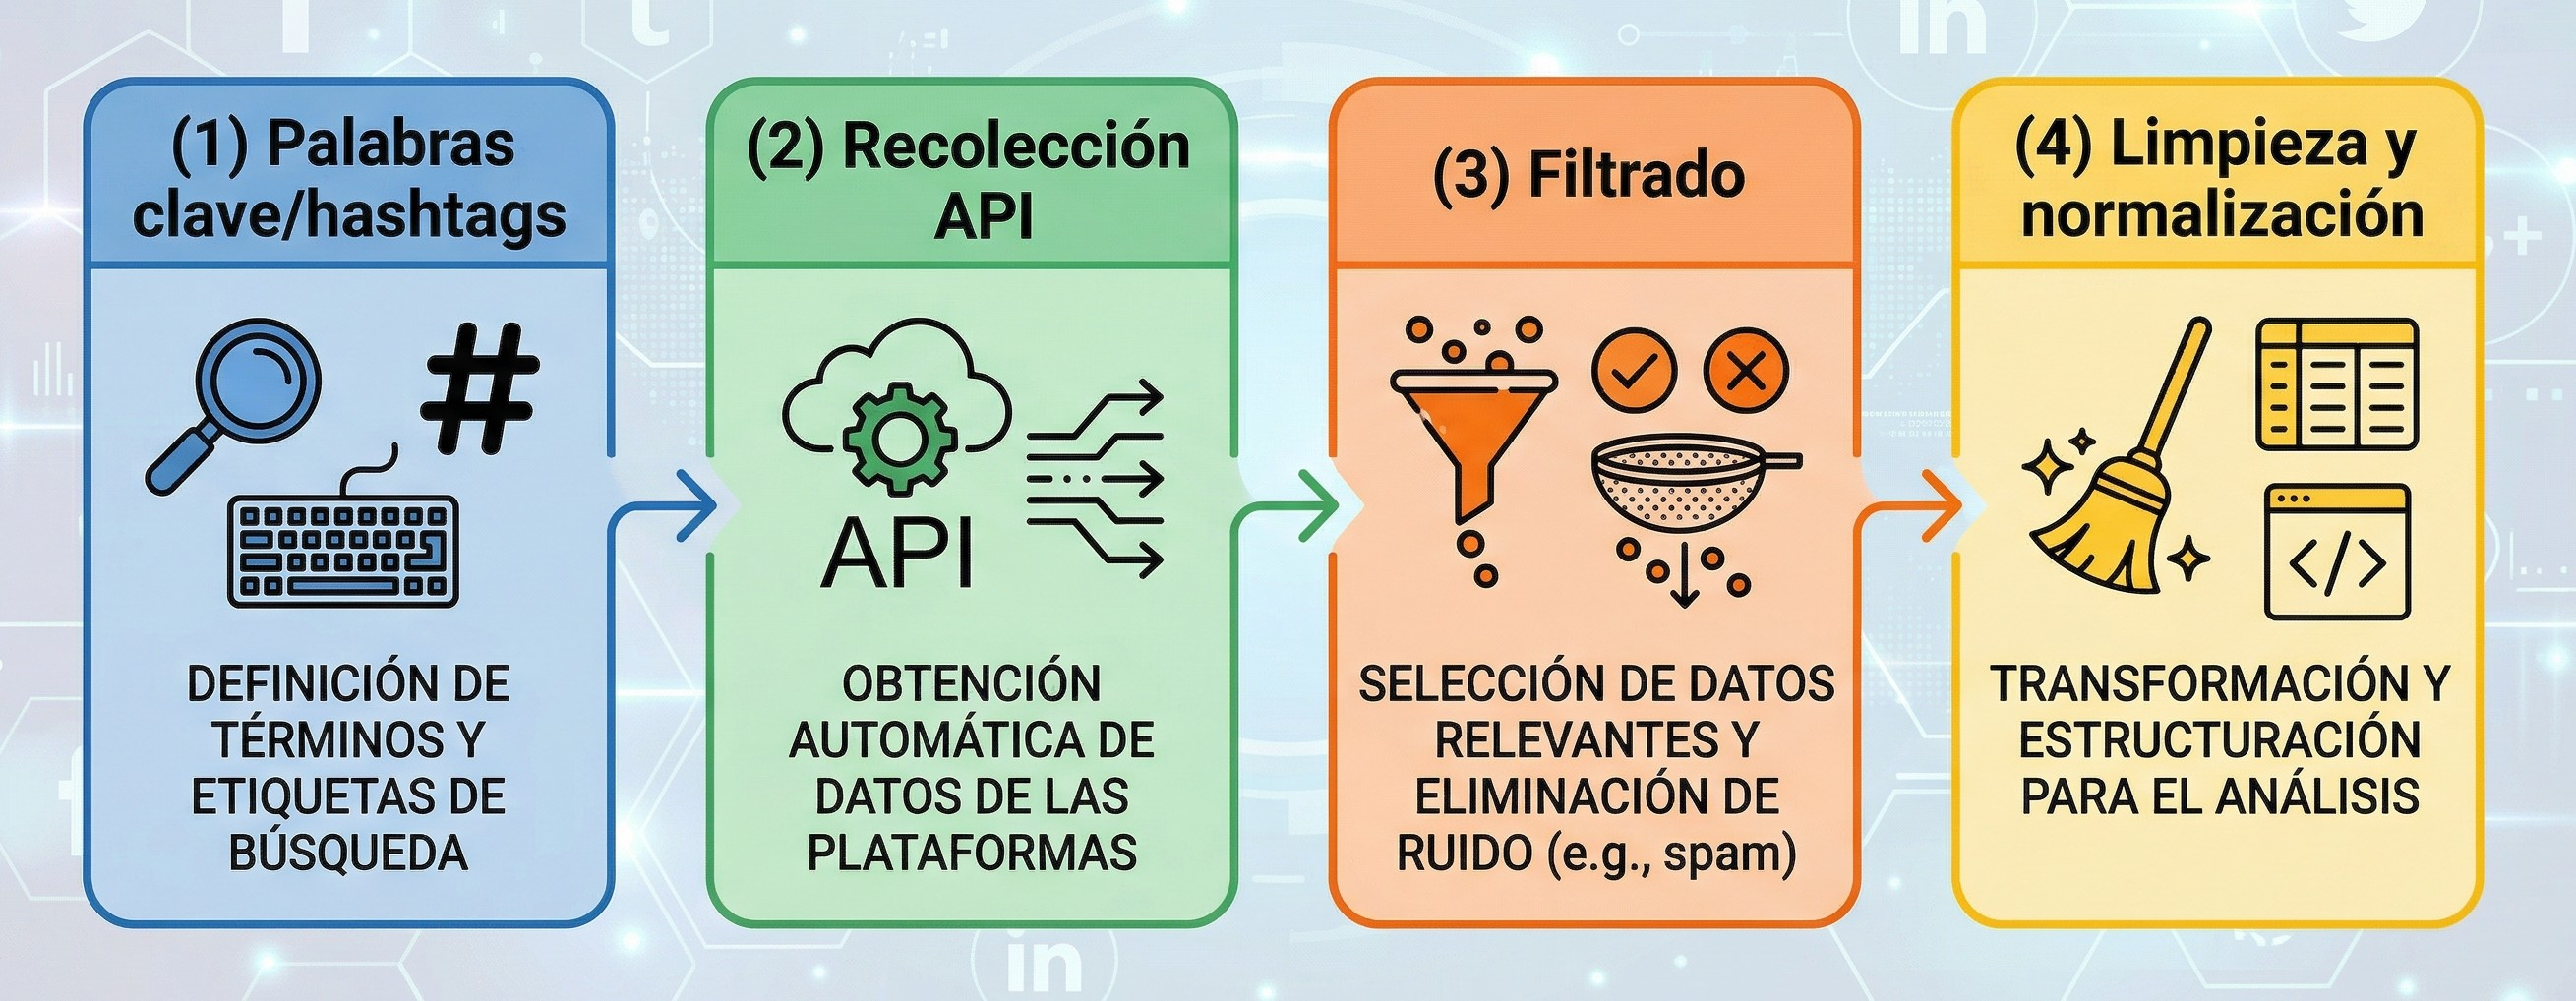
\includegraphics[width=0.85\textwidth]{2/figures/data_collection_pipeline.jpg}
        \caption[Pipeline de recolección y preprocesamiento de datos de redes sociales para análisis electoral]{Pipeline estándar para la recolección y preprocesamiento de datos de redes sociales destinados al análisis de percepción política: definición de palabras clave, recolección vía API, filtrado, limpieza y normalización del texto.\\
            Fuente: Elaboración propia basada en \cite{pr_alvi2023twitter_election_review}.}
        \label{fig:data_collection_pipeline}
    \end{center}
\end{figure}
 
El proceso comprende las siguientes etapas: (1) \textbf{Definición de criterios de búsqueda}: selección de palabras clave, hashtags y cuentas de interés relacionadas con el proceso electoral a monitorear. (2) \textbf{Recolección vía API}: extracción de publicaciones mediante las APIs oficiales de las plataformas o herramientas de scraping. (3) \textbf{Filtrado}: eliminación de publicaciones irrelevantes, spam y bots. (4) \textbf{Limpieza y normalización}: eliminación de caracteres especiales, URLs, emojis no relevantes y normalización ortográfica.
 
\subsubsection{Detección de Desinformación en Ecosistemas Digitales}
 
Un desafío crítico en el análisis de percepción pública en ecosistemas digitales es la presencia de \textbf{desinformación} (\textit{misinformation} y \textit{disinformation}): contenido falso o engañoso que circula masivamente en redes sociales con el potencial de distorsionar la percepción ciudadana y los resultados electorales \parencite{pr_chen2024combating_misinformation}. Los LLMs representan un arma de doble filo en este contexto: por un lado, son capaces de generar contenido falso de alta calidad y difícil detección; por otro, ofrecen capacidades avanzadas de verificación automática de hechos y detección de narrativas engañosas que superan los métodos tradicionales.
 
% ──────────────────────────────────────────────────────────────
\subsection{Inteligencia Electoral}
% ──────────────────────────────────────────────────────────────
 
La \textbf{inteligencia electoral} es un campo emergente que integra técnicas de ciencia de datos, NLP e inteligencia artificial para analizar, interpretar y anticipar dinámicas del comportamiento político ciudadano a partir de múltiples fuentes de información \parencite{tec_ceron2017social}. Va más allá del simple monitoreo de redes sociales al incorporar capacidades de análisis semántico profundo, detección de patrones, seguimiento de narrativas en el tiempo y correlación con indicadores externos como encuestas de opinión y resultados electorales históricos.
 
Un sistema de inteligencia electoral integrado, como el propuesto en la presente investigación, articula los siguientes componentes, cuya interacción se ilustra en la Figura \ref{fig:electoral_intelligence_system}:
 
\begin{figure}[!ht]
    \begin{center}
        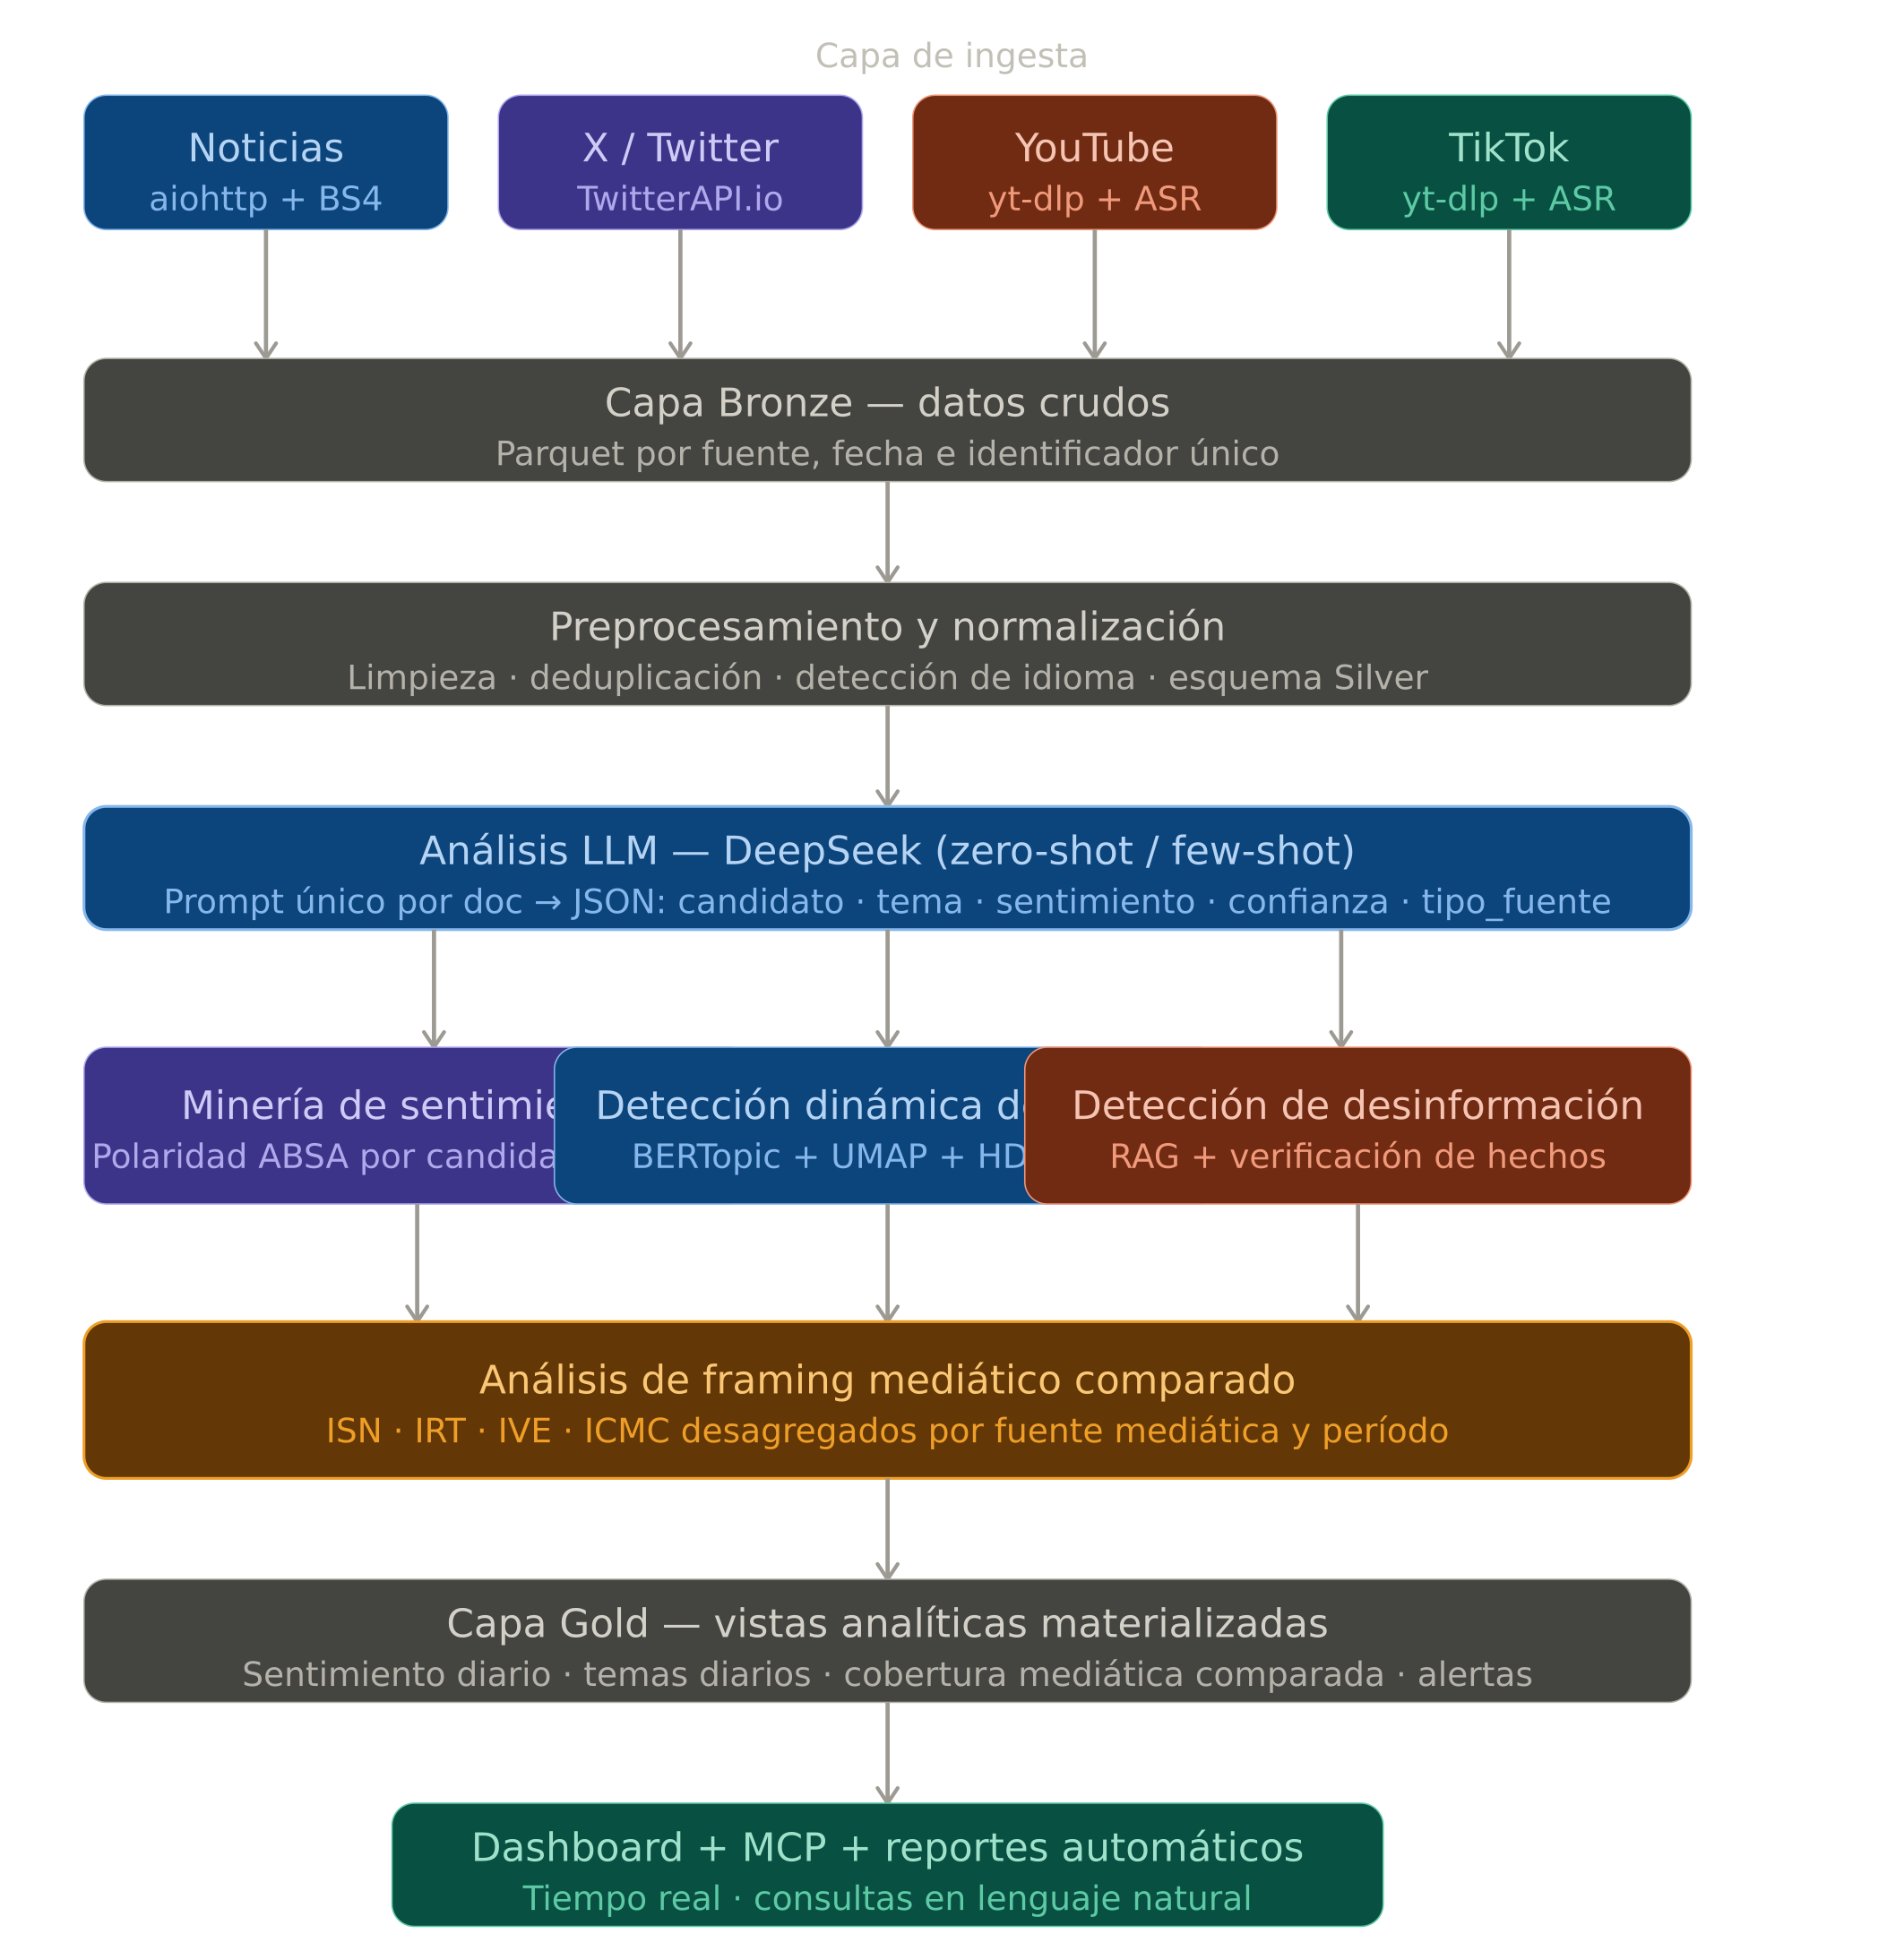
\includegraphics[width=0.90\textwidth]{2/figures/electoral_intelligence_system.jpg}
        \caption[Arquitectura de un sistema integrado de inteligencia electoral basado en LLMs]{Arquitectura de un sistema integrado de inteligencia electoral: recolección de datos multicanal, preprocesamiento, análisis de sentimientos con LLMs, detección dinámica de temas, detección de desinformación y visualización en tiempo real.\\
            Fuente: Elaboración propia.}
        \label{fig:electoral_intelligence_system}
    \end{center}
\end{figure}
 
\begin{itemize}
    \item \textbf{Recolección de datos multicanal}: ingesta en tiempo real de publicaciones de redes sociales, noticias digitales y foros de discusión ciudadana.
    \item \textbf{Análisis de sentimientos con LLMs}: clasificación de la polaridad (positivo, negativo, neutral) y la emoción asociada a cada publicación, desagregada por actores políticos y temas.
    \item \textbf{Detección dinámica de temas}: identificación automática y seguimiento temporal de los temas relevantes en la conversación política nacional.
    \item \textbf{Detección de desinformación}: identificación de contenido potencialmente falso o engañoso mediante técnicas de verificación basadas en LLMs.
    \item \textbf{Visualización y reporting}: dashboards interactivos que permiten a analistas políticos, periodistas e investigadores explorar los resultados del sistema en tiempo real.
\end{itemize}
 
\subsubsection{Medición de la Percepción Pública Nacional}
 
La \textbf{percepción pública nacional} en el contexto electoral se refiere al conjunto de actitudes, opiniones y emociones que los ciudadanos expresan colectivamente —en especial en ecosistemas digitales— hacia candidatos, partidos políticos, propuestas programáticas e instituciones democráticas. Su medición mediante LLMs ofrece ventajas sustanciales respecto a las encuestas tradicionales: es continua (no puntual), de bajo costo, capaz de procesar millones de expresiones ciudadanas simultáneamente y de detectar cambios bruscos de opinión asociados a eventos específicos de la campaña \parencite{pr_gujral2024llm_elections}.
 
Sin embargo, es importante reconocer sus limitaciones metodológicas: la representatividad del universo digital no es idéntica al electorado real, y los sesgos de los datos de entrenamiento de los LLMs pueden introducir distorsiones sistemáticas en las clasificaciones de sentimiento hacia ciertos actores políticos \parencite{pr_gujral2024llm_elections}. La triangulación con otras fuentes de datos y la interpretación crítica de los resultados son, por tanto, componentes indispensables de cualquier sistema de inteligencia electoral responsable.